\section{Papers With Code (SOTA Platform)}
{{\footnotesize
\begin{description}[labelwidth=5em, labelsep=1em, leftmargin=*, align=left, itemsep=0.3em, parsep=0em]
  \item[date:] ongoing
  \item[version:] TODO
  \item[last\_updated:] 2025-06
  \item[expired:] unknown
  \item[valid:] yes
  \item[valid\_date:] TODO
  \item[url:] \href{https://paperswithcode.com/sota}{https://paperswithcode.com/sota}
  \item[doi:] TODO
  \item[domain:] General ML; All domains
  \item[focus:] Open platform tracking state-of-the-art results, benchmarks, and implementations across ML tasks and papers
  \item[keywords:]
    - leaderboard
    - benchmarking
    - reproducibility
    - open-source
  \item[summary:] Papers With Code (PWC) aggregates benchmark suites, tasks, and code across ML research:
12,423 benchmarks, 5,358 unique tasks, and 154,766 papers with code links. It tracks SOTA metrics and fosters reproducibility.

  \item[licensing:] TODO
  \item[task\_types:]
    - Multiple (Classification, Detection, NLP, etc.)
  \item[ai\_capability\_measured:]
    - Model performance across tasks (accuracy
    - F1
    - BLEU
    - etc.)
  \item[metrics:]
    - Task-specific (Accuracy, F1, BLEU, etc.)
  \item[models:]
    - All published models with code
  \item[ml\_motif:]
    - Multiple
  \item[type:] Platform
  \item[ml\_task:]
    - Multiple
  \item[solutions:] TODO
  \item[notes:] Community-driven open platform; automatic data extraction and versioning.

  \item[contact.name:] Papers With Code Team
  \item[contact.email:] unknown
  \item[results.links.name:] ChatGPT LLM
  \item[fair.reproducible:] Yes
  \item[fair.benchmark\_ready:] Yes
  \item[ratings.software.rating:] 0
  \item[ratings.software.reason:] Not analyzed.

  \item[ratings.specification.rating:] 9.0
  \item[ratings.specification.reason:] Evaluation setting (federated clinical benchmarking) is well-defined; I/O interfaces vary slightly by task but are standardized in MedPerf platform.

  \item[ratings.dataset.rating:] 8.0
  \item[ratings.dataset.reason:] Uses distributed, real-world clinical datasets across institutions; FAIR compliance varies across hospitals and data hosts.

  \item[ratings.metrics.rating:] 9.0
  \item[ratings.metrics.reason:] ROC AUC, accuracy, and fairness metrics are explicitly defined and task-dependent; consistently tracked across institutions.

  \item[ratings.reference\_solution.rating:] 8.0
  \item[ratings.reference\_solution.reason:] Validated CNNs and GaNDLF pipelines are used and shared via the MedPerf tool, but some implementations are abstracted behind the platform.

  \item[ratings.documentation.rating:] 9.0
  \item[ratings.documentation.reason:] Excellent documentation across MedPerf, GaNDLF, and COFE; reproducibility handled via containerized flows and task templates.

  \item[id:] papers\_with\_code\_sota\_platform
  \item[Citations:] \cite{pmlr-v37-blum15}
  \item[Ratings:]
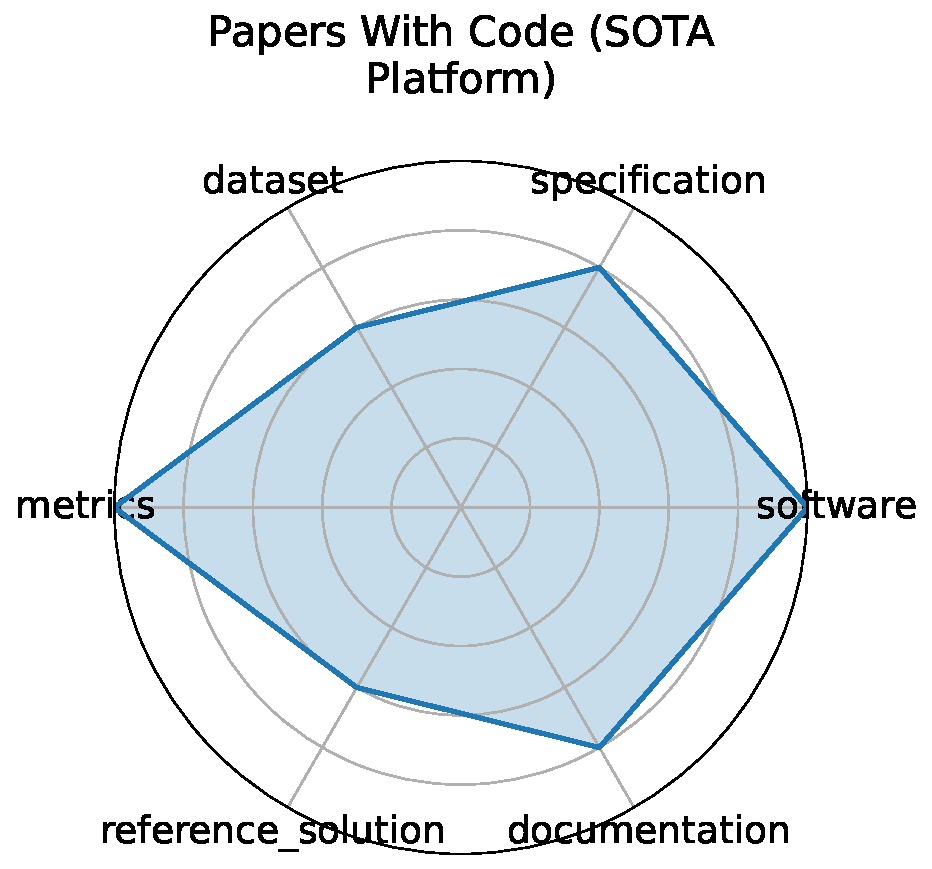
\includegraphics[width=0.2\textwidth]{papers_with_code_sota_platform_radar.pdf}
\end{description}
}}
\clearpage